\section{Multiplicación de matrices}

Se acabó lo que se daba. \textit{This is the end.}

Se nos pide escribir un \textit{kernel}\footnote{
No confundir con un \href{https://en.wikipedia.org/wiki/Kernel}{\textit{kernel}}.}\footnote{
Tampoco con \textit{Kernel}, el antiguo gato de la \href{https://etsiit.ugr.es}{ETSIIT}.}
que realize el producto de \href{http://matrices.net/tutorials.htm}{Matrices}.


Ilusionados, llenos de energía asi como de melancolía, comenzamos la resolución del ejercicio.

\subsection{Primera versión.}

Nos ponemos como objetivo acabar con un algoritmo correcto de forma que utilice
hebras y bloques independientemente de su eficiencia.

\begin{figure}[H]
    \centering
    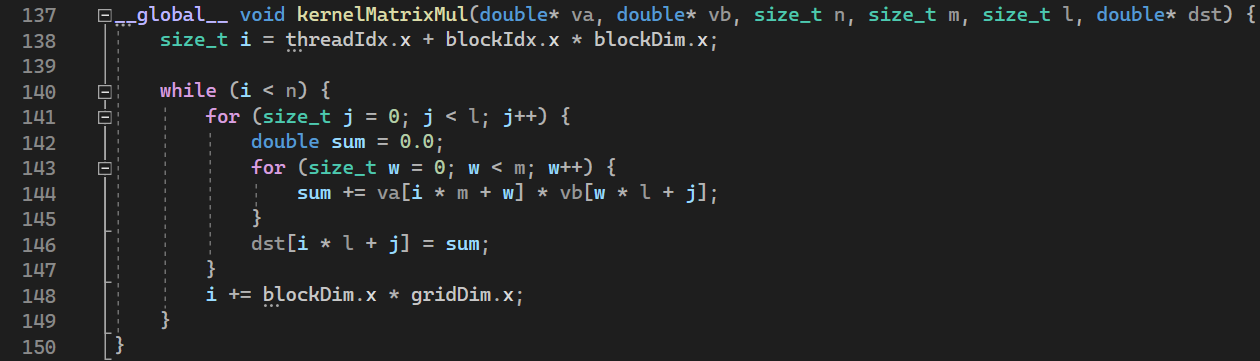
\includegraphics[width=\textwidth]{kernel1.png}
    \caption{Código de nuestro kernel para la primera versión. Únicamente considera que sea correcto.
    Cada hebra se encarga de una fila de la matriz que multiplica por la izquierda.}
\end{figure}

Conseguimos un factor de aceleración de x2 con respecto al algoritmo que ejecutamos en la CPU el cual no tiene consideraciones de optimización
adicionales. Para la medición tenemos en cuenta los tiempos de transferencia.

\begin{figure}[H]
    \centering
    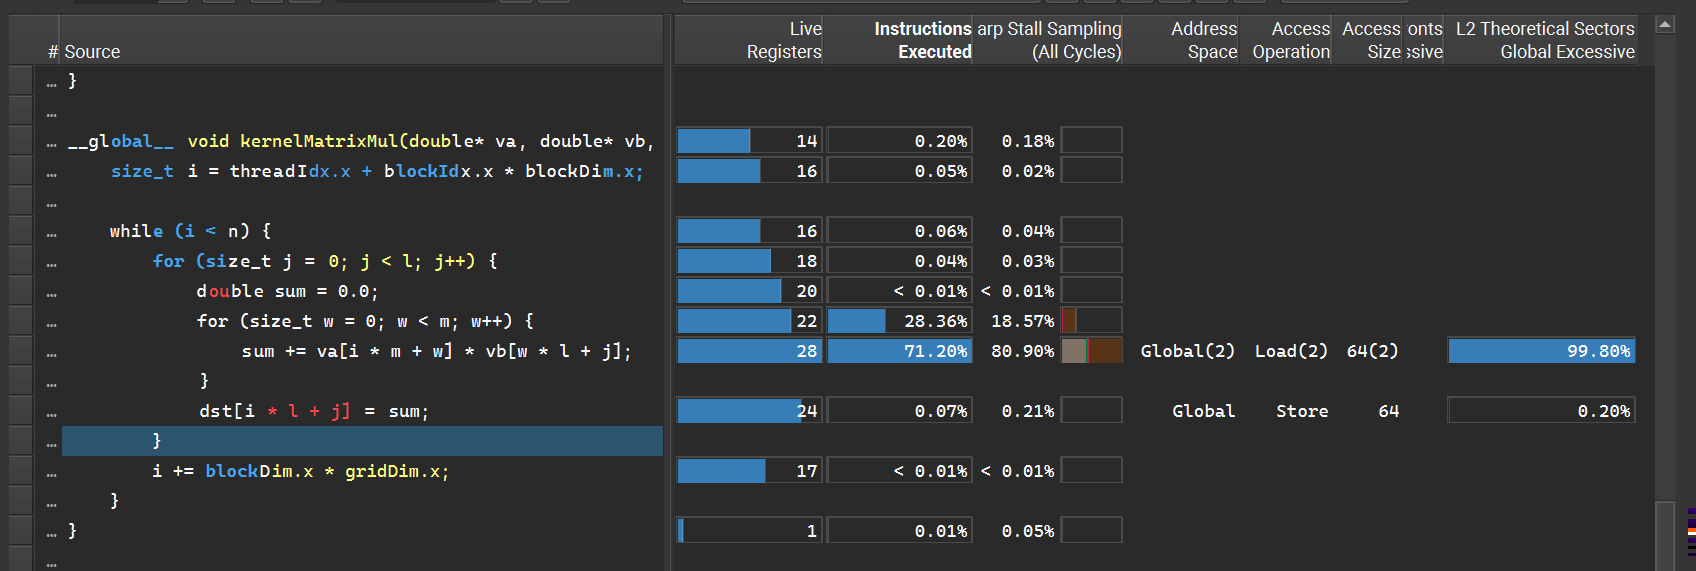
\includegraphics[width=\textwidth]{kernel1_bench.png}
    \caption{Analizador \textit{inline} de la herramienta \textit{NVIDIA NSight Compute}. Observamos cómo la mayor
    parte del esfuerzo computacional consiste tanto en acceder a memoria como en realizar la operacion de multiplicación y suma.}
\end{figure}

Tras analizar el algoritmo descubrimos que en nuestra GPU terminamos aproximadamente con un \textit{96\%} de fallos de caché de 
primer nivel y un \textit{22\%} de segundo.

\subsection{Segunda versión.}

Una vez terminada, probada y medida la primera versión iteramos sobre esta. Nuestro objetivo ahora será optimizar los
accesos a memoria.

La razón de elegir este como nuestro objetivo es que a nivel de \textit{warp}, si una hebra no puede recuperar memoria
todas las hebras de este, quedan a la espera. Es uno de los factores determinantes que dictan la ocupación de nuestra \textit{GPU}.

\begin{figure}[H]
    \centering
    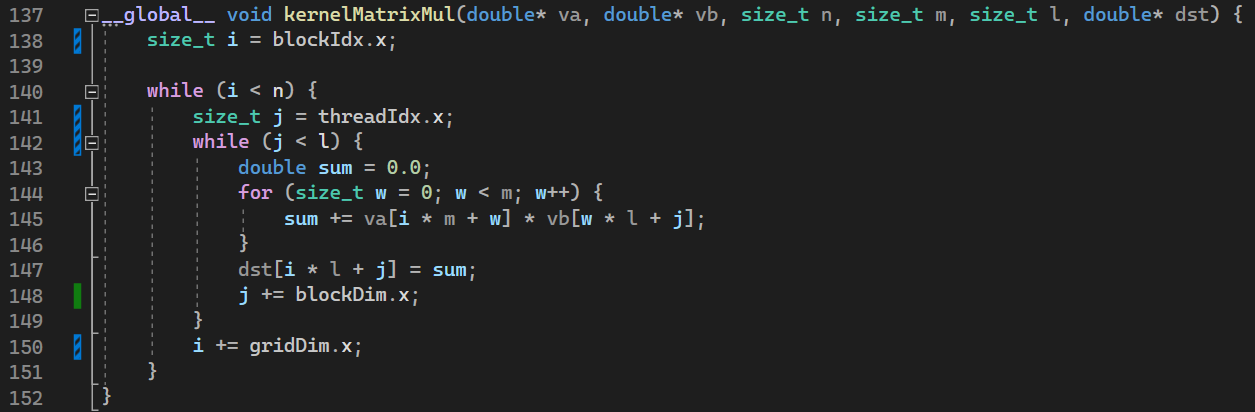
\includegraphics[width=\textwidth]{kernel2.png}
    \caption{Código de nuestro kernel para la segunda versión. Hacemos que cada bloque de hebras se encargue de una fila
    de la matriz que multiplica por la izquierda, favoreciendo la localidad especial, e intentando que ocurra de forma
    similar cuando se acceda a cada fila de la que multiplica por la derecha.}
\end{figure}

Conseguimos un factor de aceleración de x34\footnote{Con \href{https://www.youtube.com/watch?v=uC9d34cU2s8&t=73s}{risa maligna} incluida.} con respecto al algoritmo que ejecutamos en la CPU.
Para la medición tenemos en cuenta los tiempos de transferencia.

\begin{figure}[H]
    \centering
    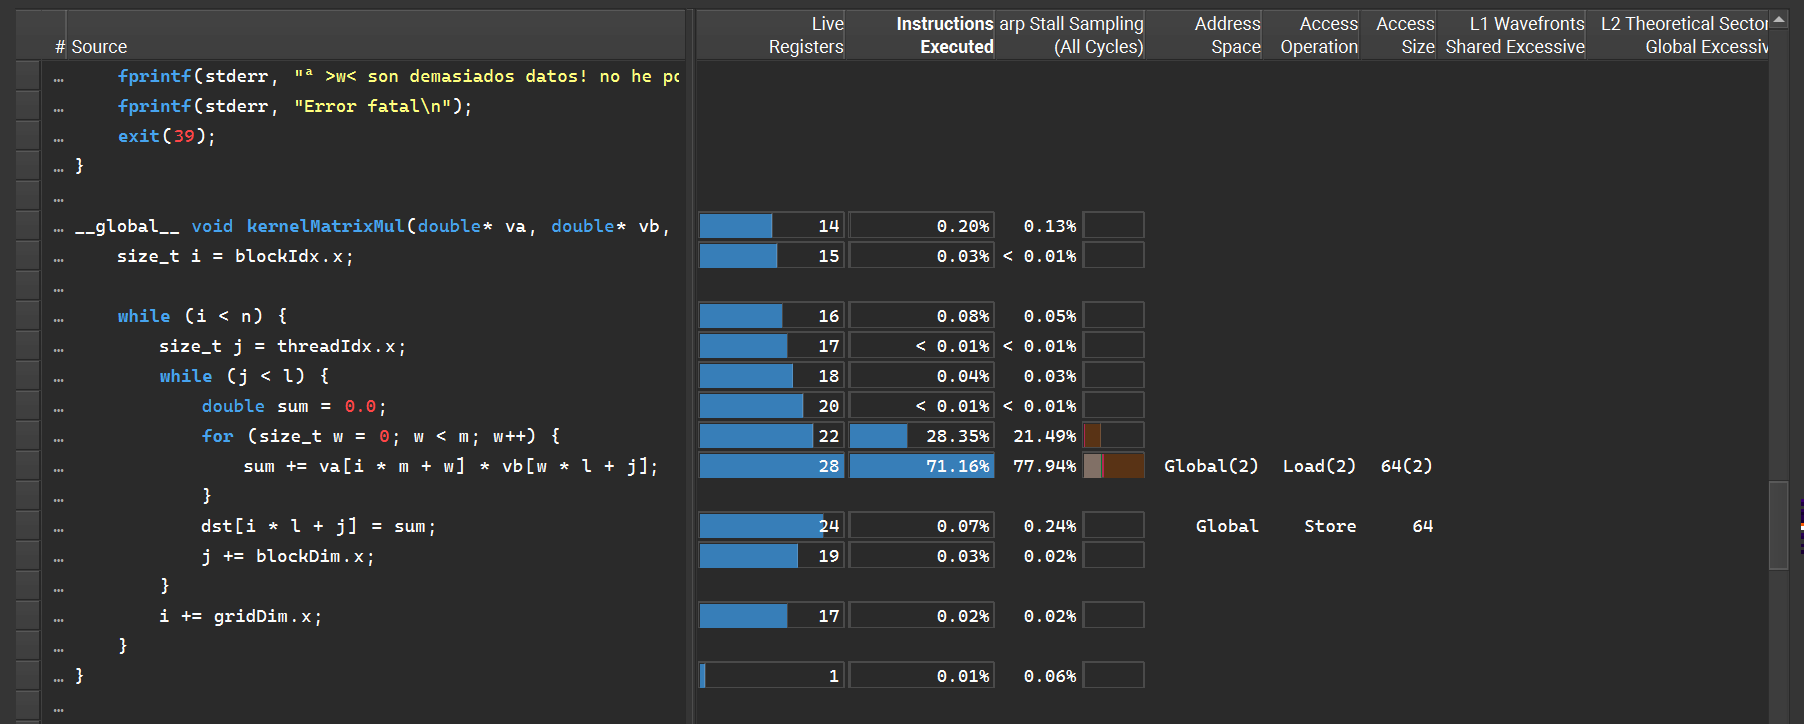
\includegraphics[width=\textwidth]{kernel2_bench.png}
    \caption{Analizador \textit{inline} de la herramienta \textit{NVIDIA NSight Compute}. Conseguimos que nuestra GPU tenga un \textit{94\%} de aciertos de caché al segundo
    nivel y un \textit{57.9\%} al primer nivel.}
\end{figure}

A lo mejor no tendremos segunda cita, pero lo cierto es que ya conoces lo penalizante que es realizar
accesos a memoria al \textit{tun-tún}.\footnote{Basado en un meme que ahora mismo no encuentro.}

\subsection{Alternativas y trabajo futuro.}

Si nuestro objetivo fuese seguir aprendiendo seguramente seguiríamos la entrada de blog que encontramos en \href{https://siboehm.com/articles/22/CUDA-MMM}{el siguiente enlace}.

Por otra parte, si quisiésemos acelerar la multiplicación de matrices en nuestro código utilizaríamos una librería como \href{https://docs.nvidia.com/cuda/cublas/}{cuBLAS}

Fin.
